% \documentclass[table]{beamer}
\documentclass[table,handout]{beamer}
\setbeameroption{show notes}
% \setbeameroption{hide notes}
% \setbeameroption{show only notes}
\usepackage{varwidth}

\newif\ifhide
\newif\ifpost
\newif\ifhideclicker

% \hidetrue
% \hideclickertrue
% \posttrue

\newcommand{\whiteout}[1]{\textcolor{white}{#1}}
% \newcommand{\whiteoutbox}[1]{\fcolorbox{white}{white}{\parbox{\dimexpr \linewidth-2\fboxsep-2\fboxrule}{\whiteout{#1}}}}
% \newcommand{\notebox}[1]{\fcolorbox{blue}{white}{\parbox{\dimexpr \linewidth-2\fboxsep-2\fboxrule}{#1}}}
\newcommand{\whiteoutbox}[1]{\fcolorbox{white}{white}{\parbox{\linewidth}{\whiteout{#1}}}}
\newcommand{\notebox}[1]{\fcolorbox{blue}{white}{\parbox{\linewidth}{#1}}}
\newcommand{\blankbox}[1]{\phantom{\varwidth{\linewidth}\whiteoutbox{#1}\endvarwidth}}
\newcommand{\blank}[1]{\phantom{\varwidth{\linewidth}#1\endvarwidth}}

\ifhide%
    \newcommand{\hmask}[1]{\blank{#1}}%
\else%
    \newcommand{\hmask}[1]{#1}%
\fi

\ifhide%
    \newcommand{\wout}[1]{\whiteout{#1}}%
\else%
    \newcommand{\wout}[1]{#1}%
\fi

\ifhide%
    \newcommand{\hignore}[1]{}%
\else%
    \newcommand{\hignore}[1]{#1}%
\fi

\ifpost%
    \newcommand{\nopost}[1]{}%
\else%
    \newcommand{\nopost}[1]{#1}%
\fi

\ifhideclicker%
    \newcommand{\clickerslide}[1]{\stepcounter{clickerQuestionCounter}%
        \begin{frame}[t]
            \textcolor{blue}{Q \arabic{clickerQuestionCounter}:}
        \end{frame}}
\else%
    \newcommand{\clickerslide}[1]{#1}%
\fi

\ifhide%
    \newcommand{\hidebox}[1]{\blank{#1}}%
\else%
    \newcommand{\hidebox}[1]{\notebox{#1}}%
\fi

\ifhide%
    \newcommand{\wbox}[1]{\whiteoutbox{#1}}%
\else%
    \newcommand{\wbox}[1]{\notebox{#1}}%
\fi

\ifhide%
    \newcommand{\nbox}[1]{\blankbox{#1}}%
\else%
    \newcommand{\nbox}[1]{\notebox{#1}}%
\fi

\ifhideclicker%
    \newcommand{\clickeranswer}[1]{#1}%
\else%
    \ifhide%
        \newcommand{\clickeranswer}[1]{#1}%
    \else%
        \newcommand{\clickeranswer}[1]{\textbf{\textcolor{blue}{#1}}}%
    \fi
\fi

\usepackage{beamerthemesplit}
% \usetheme{boxes}
\usetheme{Malmoe}
\usecolortheme{seahorse}
% \usecolortheme{seagull}
\usepackage{ifthen}
\usepackage{xspace}
\usepackage{multirow}
\usepackage{multicol}
\usepackage{booktabs}
\usepackage{xcolor}
\usepackage{wasysym}
\usepackage{comment}
\usepackage{hyperref}
\hypersetup{pdfborder={0 0 0}, colorlinks=true, urlcolor=blue, linkcolor=blue, citecolor=blue}
\usepackage{changepage}
\usepackage[compatibility=false]{caption}
\captionsetup[figure]{font=scriptsize, labelformat=empty, textformat=simple, justification=centering, skip=2pt}
\usepackage{tikz}
\usetikzlibrary{trees,calc,backgrounds}

\usepackage[bibstyle=joaks-slides,maxcitenames=3,mincitenames=1,backend=biber]{biblatex}

\newrobustcmd*{\shortfullcite}{\AtNextCite{\renewbibmacro{title}{}\renewbibmacro{in:}{}\renewbibmacro{number}{}}\fullcite}

\newrobustcmd*{\footlessfullcite}{\AtNextCite{\renewbibmacro{title}{}\renewbibmacro{in:}{}}\footfullcite}

% Make all footnotes smaller
% \renewcommand{\footnotesize}{\scriptsize}

\definecolor{myGray}{gray}{0.9}
\colorlet{rowred}{red!30!white}

\setbeamertemplate{blocks}[rounded][shadow=true]

\setbeamercolor{defaultcolor}{bg=structure!30!normal text.bg,fg=black}
\setbeamercolor{block body}{bg=structure!30!normal text.bg,fg=black}
\setbeamercolor{block title}{bg=structure!50!normal text.bg,fg=black}

\newenvironment<>{varblock}[2][\textwidth]{%
  \setlength{\textwidth}{#1}
  \begin{actionenv}#3%
    \def\insertblocktitle{#2}%
    \par%
    \usebeamertemplate{block begin}}
  {\par%
    \usebeamertemplate{block end}%
  \end{actionenv}}

\newenvironment{displaybox}[1][\textwidth]
{
    \centerline\bgroup\hfill
    \begin{beamerboxesrounded}[lower=defaultcolor,shadow=true,width=#1]{}
}
{
    \end{beamerboxesrounded}\hfill\egroup
}

\newenvironment{onlinebox}[1][4cm]
{
    \newbox\mybox
    \newdimen\myboxht
    \setbox\mybox\hbox\bgroup%
        \begin{beamerboxesrounded}[lower=defaultcolor,shadow=true,width=#1]{}
    \centering
}
{
    \end{beamerboxesrounded}\egroup
    \myboxht\ht\mybox
    \raisebox{-0.25\myboxht}{\usebox\mybox}\hspace{2pt}
}

\newenvironment{mydescription}{
    \begin{description}
        \setlength{\leftskip}{-1.5cm}}
    {\end{description}}

\newenvironment{myitemize}{
    \begin{itemize}
        \setlength{\leftskip}{-.3cm}}
    {\end{itemize}}

% footnote without a marker
\newcommand\barefootnote[1]{%
  \begingroup
  \renewcommand\thefootnote{}\footnote{#1}%
  \addtocounter{footnote}{-1}%
  \endgroup
}

% define formatting for footer
\newcommand{\myfootline}{%
    {\it
    \insertshorttitle
    \hspace*{\fill} 
    \insertshortauthor, \insertshortinstitute
    % \ifx\insertsubtitle\@empty\else, \insertshortsubtitle\fi
    \hspace*{\fill}
    \insertframenumber/\inserttotalframenumber}}

% set up footer
\setbeamertemplate{footline}{%
    \usebeamerfont{structure}
    \begin{beamercolorbox}[wd=\paperwidth,ht=2.25ex,dp=1ex]{frametitle}%
        % \Tiny\hspace*{4mm}\myfootline\hspace{4mm}
        \tiny\hspace*{4mm}\myfootline\hspace{4mm}
    \end{beamercolorbox}}

% remove navigation bar
\beamertemplatenavigationsymbolsempty

\makeatletter
    \newenvironment{noheadline}{
        \setbeamertemplate{headline}[default]
        \def\beamer@entrycode{\vspace*{-\headheight}}
    }{}
\makeatother

\newcounter{clickerQuestionCounter}
\ifhideclicker%
\newenvironment{clickerquestion}
{ \stepcounter{clickerQuestionCounter}
  \begin{enumerate}[Q \arabic{clickerQuestionCounter}:]\color{white} }
{ \end{enumerate} }
\else%
\newenvironment{clickerquestion}
{ \stepcounter{clickerQuestionCounter}
  \begin{enumerate}[Q \arabic{clickerQuestionCounter}:] }
{ \end{enumerate} }
\fi

\ifhideclicker%
\newenvironment{clickeroptions}
{ \begin{enumerate}[\begingroup\color{white} 1)\endgroup]\color{white} }
{ \end{enumerate} }
\else%
\newenvironment{clickeroptions}
{ \begin{enumerate}[\begingroup\color{red} 1)\endgroup] }
{ \end{enumerate} }
\fi


\tikzstyle{centered} = [align=center, text centered, font=\sffamily\bfseries]
\tikzstyle{skip} = [centered, inner sep=0pt, fill]
\tikzstyle{empty} = [centered, inner sep=0pt]
\tikzstyle{inode} = [centered, circle, minimum width=4pt, fill=black, inner sep=0pt]
\tikzstyle{tnode} = [centered, circle, inner sep=1pt]
\tikzset{
  % edge styles
  level distance=10mm,
  mate/.style={edge from parent/.style={draw,distance=3pt}},
  mleft/.style={grow=left, level distance=10mm, edge from parent path={(\tikzparentnode.west)--(\tikzchildnode.east)}},
  mright/.style={grow=right, level distance=10mm, edge from parent path={(\tikzparentnode.east)--(\tikzchildnode.west)}},
  % node styles
  male/.style={rectangle,minimum size=4mm,fill=gray!80},
  female/.style={circle,minimum size=4mm,fill=gray!80},
  amale/.style={male,fill=red},
  afemale/.style={female,fill=red},
}

\newcommand{\highlight}[1]{\textcolor{violet}{\textit{\textbf{#1}}}}
\newcommand{\super}[1]{\ensuremath{^{\textrm{\sffamily #1}}}}
\newcommand{\sub}[1]{\ensuremath{_{\textrm{\sffamily #1}}}}
\newcommand{\dC}{\ensuremath{^\circ{\textrm{C}}}}
\newcommand{\tb}{\hspace{2em}}
\providecommand{\e}[1]{\ensuremath{\times 10^{#1}}}
\newcommand{\myHangIndent}{\hangindent=5mm}

\newcommand{\spp}[1]{\textit{#1}}

\newcommand\mybullet{\leavevmode%
\usebeamertemplate{itemize item}\hspace{.5em}}

\makeatletter
\newcommand*{\rom}[1]{\expandafter\@slowromancap\romannumeral #1@}
\makeatother

\newcommand{\blankslide}{{\setbeamercolor{background canvas}{bg=black}
\setbeamercolor{whitetext}{fg=white}
\begin{frame}<handout:0>[plain]
\end{frame}}}

\newcommand{\whiteslide}{
\begin{frame}<handout:0>[plain]
\end{frame}}

\newcommand{\f}[1]{\ensuremath{F_{#1}}}
\newcommand{\x}[1]{X\ensuremath{^{#1}}}
\newcommand{\y}[1]{Y\ensuremath{^{#1}}}

% Population growth macros
\newcommand{\popsize}[1]{\ensuremath{N_{#1}}}
\newcommand{\popgrowthratediscrete}[1]{\ensuremath{\lambda_{#1}}}
\newcommand{\popgrowthrate}[1]{\ensuremath{r_{#1}}}
\newcommand{\ptime}{\ensuremath{t}\xspace}

\tikzset{hide on/.code={\only<#1>{\color{white}}}}
\tikzset{
    invisible/.style={opacity=0},
    visible on/.style={alt={#1{}{invisible}}},
    alt/.code args={<#1>#2#3}{%
        \alt<#1>{\pgfkeysalso{#2}}{\pgfkeysalso{#3}}
        % \pgfkeysalso doesn't change the path
    },
}

\bibliography{../bib/references}
\author[J.\ Oaks]{
    %Jamie R.\ Oaks\inst{1}
    Jamie R.\ Oaks
}
\institute[BIOL 180]{
    \inst{}%
        BIOL 180: Introductory Biology
}



\title[Communities II: Species richness \& NPP]{Communities II: Species
    richness \& NPP}
% \date{\today}
\date{May 28, 2015}

% \setbeamertemplate{section in toc}[sections numbered]
% \setbeamertemplate{subsection in toc}[subsections numbered]

\begin{document}

\begin{noheadline}
\maketitle
\end{noheadline}

\nopost{
\begin{noheadline}
\begin{frame}[c]
    \vspace{-6mm}
    \begin{center} 
        \includegraphics[height=1.2\textheight]{../images/seating-chart-2.pdf}
    \end{center}
\end{frame}
\end{noheadline}
}

\clickerslide{
\begin{noheadline}
\begin{frame}
    \begin{clickerquestion}
        \item What type of disturbance (besides logging) is most common (in
            frequency, and in total area affected) in the forests of Western
            Washington? 

        \begin{clickeroptions}
            \item Flooding
            \item Catastrophic fires (burn everything to the ground)
            \item Low-intensity fires (burn understory only)
            \item \clickeranswer{Wind-blown trees}
            \item Landslides
        \end{clickeroptions}
    \end{clickerquestion}
\end{frame}
\end{noheadline}
}

\begin{noheadline}
\begin{frame}
\frametitle{Today's issues:}
\vspace{5mm}
% \tableofcontents[subsectionstyle=hide]
\tableofcontents
\end{frame}
\end{noheadline}

\section{How do you measure biodiversity?}

\begin{frame}[t]
    \begin{adjustwidth}{-2em}{-1.5em}
        How do you measure biodiversity?

        \begin{uncoverenv}<2->
        \begin{itemize}
            \item Genetic diversity:

                \nbox{The number and relative abundance of alleles present in
                    an population}

                \vspace{2mm}
            \item Species richness:

                \nbox{The number of species present in an area}

                \vspace{2mm}
            \item Species diversity:

                \nbox{The number and relative abundance of species present in
                    an area}

                \vspace{2mm}
            \item Functional diversity:

                \nbox{The number and relative abundance of functional groups
                    (functional group = group of species that use resources in
                    similar ways).}

                \vspace{2mm}
            \item Phylogenetic diversity:

                \nbox{The number, and phylogenetic relatedness, of species in
                    an area}
        \end{itemize}

        \centerline{
            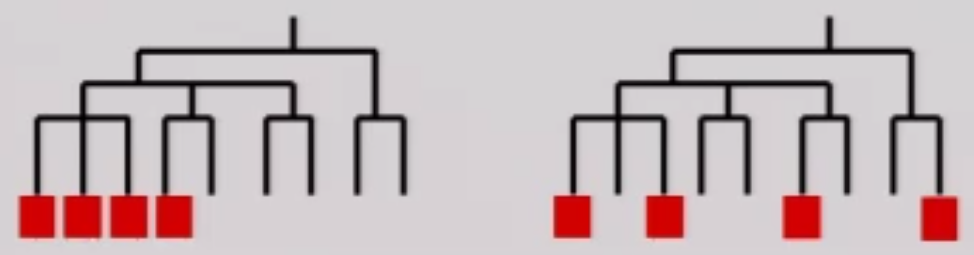
\includegraphics[height=0.1\textheight]{phylo-diversity.png}}
        \end{uncoverenv}
    \end{adjustwidth}
\end{frame}

\begin{frame}[t]
    \begin{adjustwidth}{-2em}{-1.5em}
        Does plant species richness affect productivity?

        \begin{itemize}
            \item Gross primary productivity (GPP):

                \nbox{Total amount of energy captured (transformed into
                    chemical energy) by primary producers. In most systems,
                    this is the amount of solar energy captured by
                    photosynthesis.}

            \item Net primary productivity (NPP):

                \nbox{Energy invested by primary producers in building biomass
                    (tissues or offspring). This is a fraction of GPP.}

            \item What's the difference?

                \nbox{Energy wasted and used for respiration (metabolism) by
                    primary producers (R). NPP = GPP - R}

            \item Why is NPP so important?

                \nbox{It represents the energy available to the rest of the
                    community}
        \end{itemize}

    \end{adjustwidth}
\end{frame}

\begin{frame}[t]
    \begin{adjustwidth}{-2em}{-1.5em}
        Experiments in North American prairies

        \uncover<2->{
        \vspace{4mm}
        32 species from 5 functional groups (different functional groups use or
        allocate resources in different ways).
        }

        \uncover<3->{
        \begin{enumerate}
            \item Cool season grasses---grow in spring and fall

                \vspace{4mm}
            \item Warm season grasses---grow in summer

                \vspace{4mm}
            \item Legumes---fix nitrogen via symbiotic bacteria

                \vspace{4mm}
            \item Woody plants---allocation to woody stems

                \vspace{4mm}
            \item Forbs---allocation to seeds, flowers
        \end{enumerate}
        }

    \end{adjustwidth}
\end{frame}

\begin{frame}[t]
    \begin{adjustwidth}{-2em}{-1.5em}
        Experiments in North American prairies

        \begin{itemize}
            \item 3m $\times$ 3m plots in field, each planted with 0--32
                randomly selected species, representing 0--5 functional groups.

            \item 2-years of growth; harvest aboveground tissues
        \end{itemize}

        \centerline{
            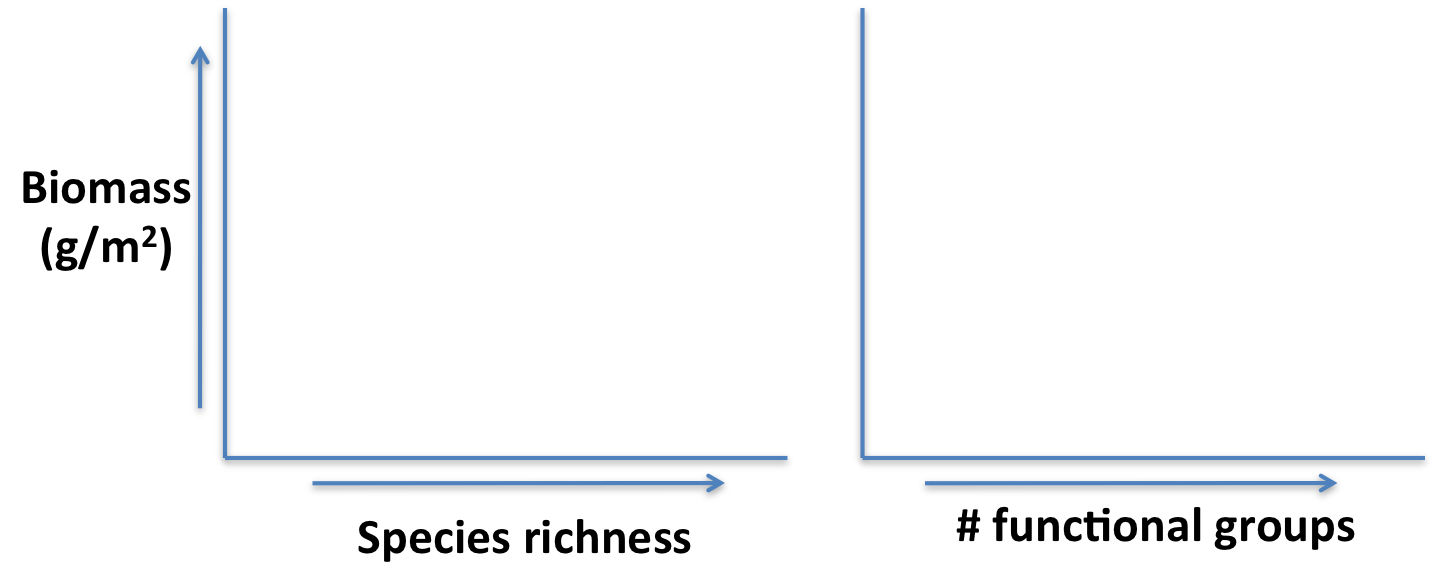
\includegraphics[width=\linewidth]{diversity-biomass-axes.png}}
        
        \nbox{\scriptsize asymptotic positive correlation for both}


    \end{adjustwidth}
\end{frame}

\clickerslide{
\begin{frame}
    \begin{clickerquestion}
        \item In most experiments where species richness is plotted on the
            x-axis and biomass on the y-axis, the curve asymptotes relatively
            quickly (often at about 10 species). What does this observation
            suggest? 
 
        \begin{clickeroptions}
            \item These experiments would be more interpretable if additional
                species were added.
            \item \clickeranswer{At some point, something besides species
                    richness limits overall productivity.}
            \item Species are like rivets in an airplane wing---losing one
                reduces function (function = NPP in this case). 
            \item The experiments haven't been run long enough. 
        \end{clickeroptions}
    \end{clickerquestion}
\end{frame}
}

\clickerslide{
\begin{frame}
    \begin{clickerquestion}
        \item It is common to observe that overall productivity increases as
            the number of species in an ecosystem increases. Which of the
            following hypotheses best explains this pattern? 

        \begin{clickeroptions}
            \item As you add more species, you are more likely to get a species
                with exceptionally high biomass production. 
            \item Different species use resources in different ways, so overall
                resource use is higher. 
            \item As you add more species, you are more likely to see
                beneficial interactions that increase overall biomass
                production.
            \item \clickeranswer{All of the above are legitimate hypotheses,
                    and they are not mutually exclusive.}
        \end{clickeroptions}
    \end{clickerquestion}
\end{frame}
}

\begin{frame}[t]
    \begin{adjustwidth}{-2em}{-1.5em}
        Potential mechanisms to explain the increase in NPP with increasing
        biodiversity:

        \begin{itemize}
            \item Sampling effect:

                \nbox{Assumption: a few ``big-producer'' species are key to
                    overall NPP. When more species are present, there is a
                    higher probability that one or more of them is a ``big
                    producer.'' I.e., with more species, you are more likely to
                    ``sample'' a big producer.}

            \item Resource use efficiency:

                \nbox{Different species use resources in different ways, and so
                    having more species present ensures that more resources are
                    used overall, and thus more productivity is possible.
                    E.g., different plants extract water and nutrients from the
                    soil at different depths.}

            \item Facilitation:

                \nbox{Some species/functional groups facilitate the growth of
                    other species/functional groups. E.g., the biomass of
                    nitrogen-fixing species provides usable forms of N
                    (``fertilizer'') for other species. With more species,
                    there are more interactions, and so there are more
                    opportunities for such beneficial interactions.}
        \end{itemize}

    \end{adjustwidth}
\end{frame}

\clickerslide{
\begin{frame}
    \begin{clickerquestion}
        \item Compared to the species richness data, what pattern would you
            expect from an experiment testing how increased genetic diversity
            (within a single species) affects productivity?
        \begin{clickeroptions}
            \item \clickeranswer{Similar (positive) relationship, because
                    similar mechanisms are relevant to allelic diversity.}
            \item Different relationship, because interspecific diversity
                is greater than intraspecific.
            \item No relationship, because these mechanisms do not occur within
                species.
            \item It would depend on which species were included and how they
                interact with each other.
        \end{clickeroptions}
    \end{clickerquestion}
\end{frame}
}

\begin{frame}[t]
    \begin{adjustwidth}{-2em}{-1.5em}
        \centerline{
            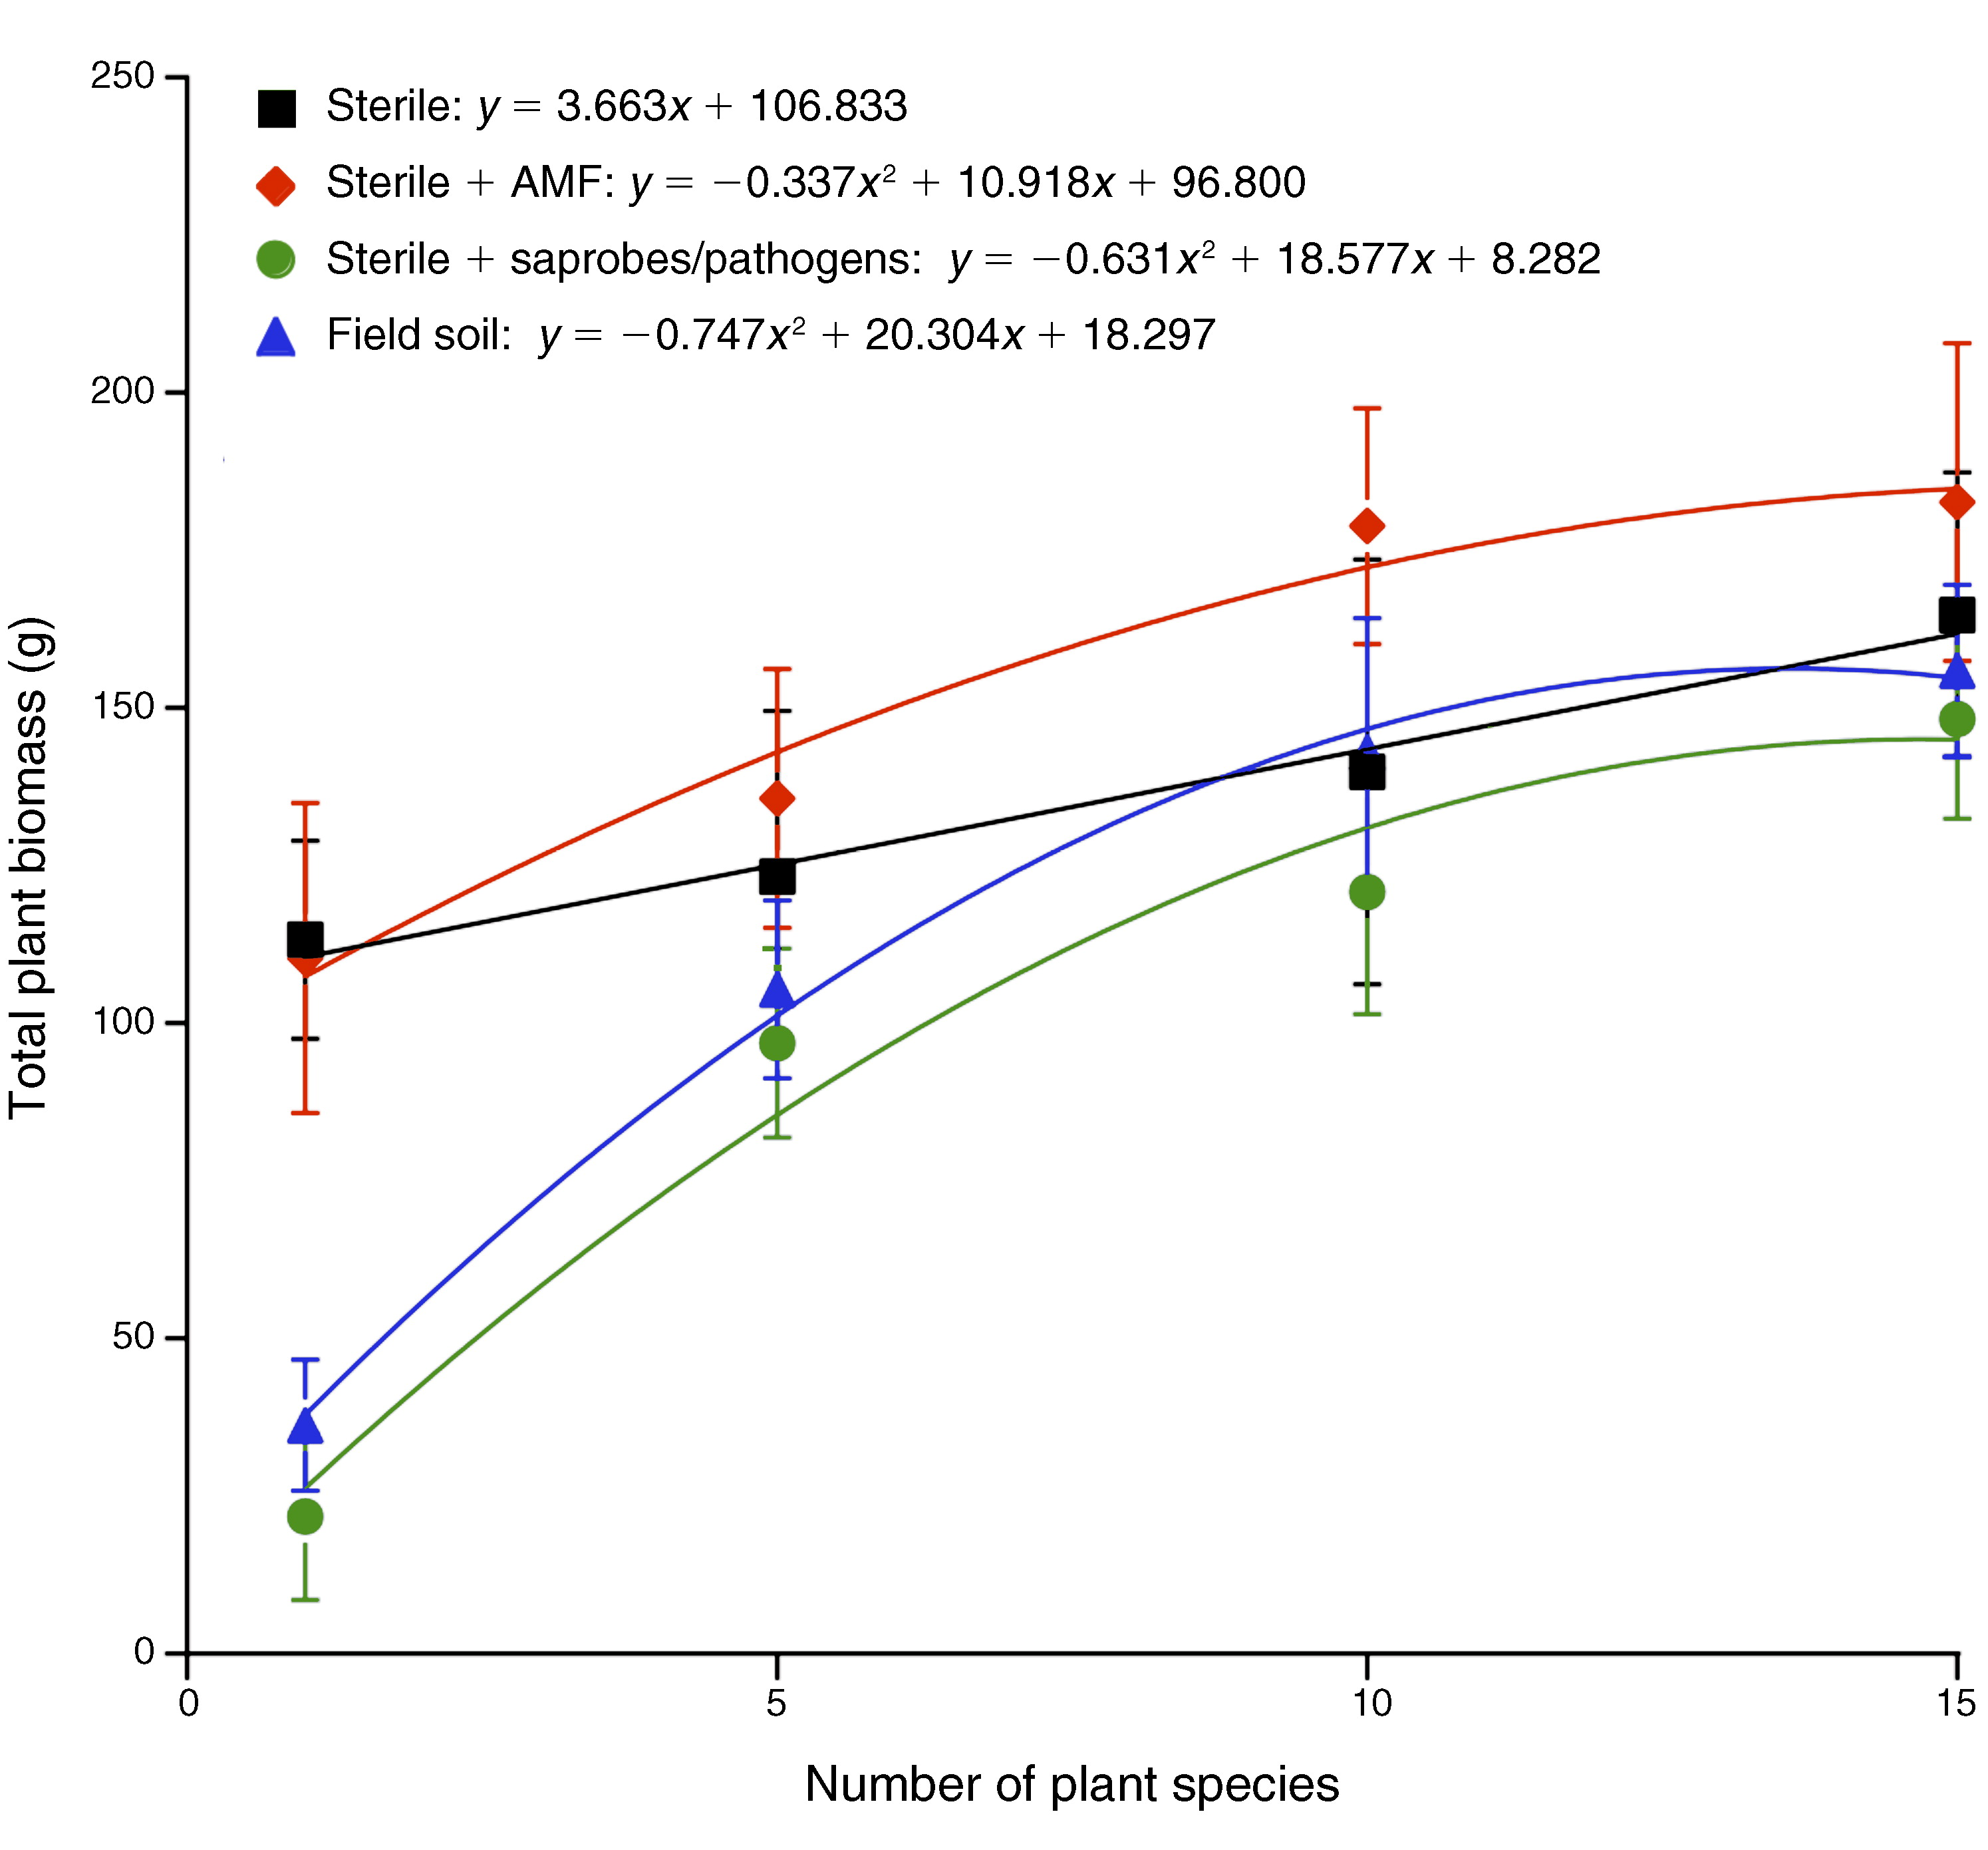
\includegraphics[width=\linewidth]{disease-community-productivity.jpg}}

        \nbox{Take-homes: (1) Communities with low species richness are much
            more affected (negatively) by disease. (2) Communities with low
            species richness show little/no benefit from mutualists.}
        \barefootnote{\shortfullcite{Schnitzer2011}}
    \end{adjustwidth}
\end{frame}

\section[Does species richness affect community function?]{Is species richness
    an important factor in how communities function?}

\section{Does biodiversity matter?}

\end{document}

\clickerslide{
\begin{frame}
    \begin{clickerquestion}
        \item 
        \begin{clickeroptions}
            \item 
            \item 
            \item 
            \item 
        \end{clickeroptions}
    \end{clickerquestion}
\end{frame}
}

\clickerpost{
{
\usebackgroundtemplate{\includegraphics[page=17,width=\paperwidth]{./24-Radiation-extinction.pdf}}
\begin{frame}[t,plain]
    \begin{adjustwidth}{-2em}{-1.5em}
        \cmask{Answer: 3}
    \end{adjustwidth}
\end{frame}
}
}

